\documentclass[margin=10pt]{standalone}
\usepackage[T1]{fontenc}
\usepackage[utf8]{inputenc}
\usepackage{pgf,tikz}
\usetikzlibrary{decorations.pathreplacing,calligraphy}

\begin{document}

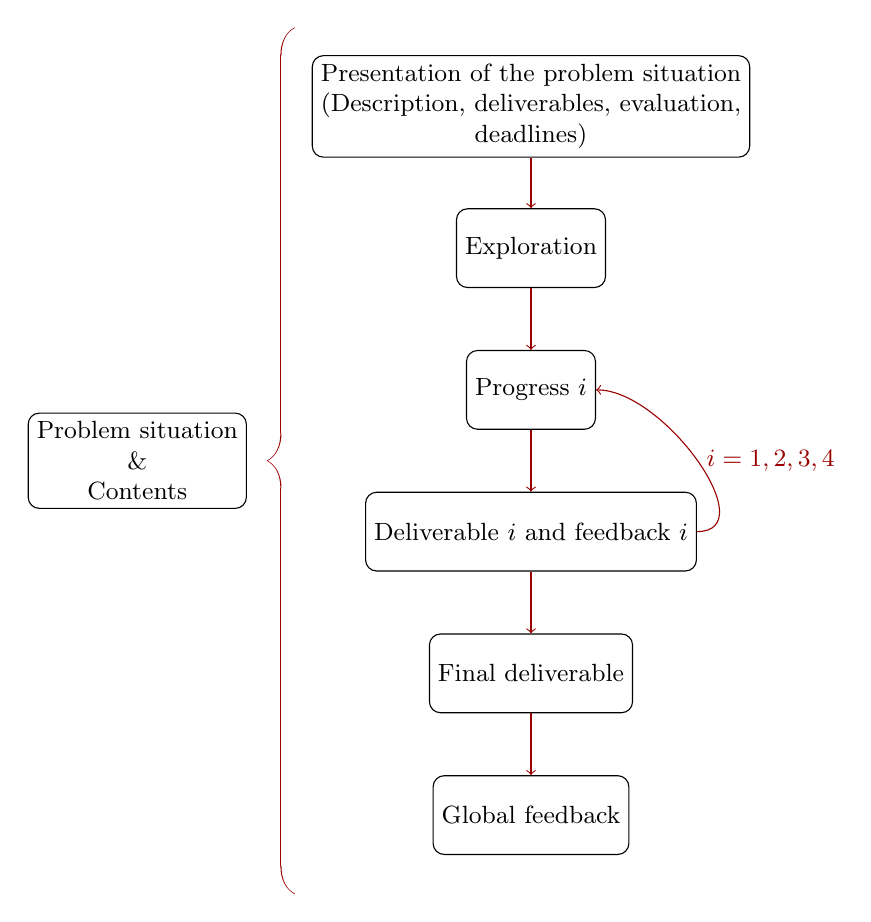
\begin{tikzpicture}[block/.style={rectangle, draw, rounded corners, minimum width=12mm, minimum height=10mm, align=center},
  sumnode/.style={circle, draw, inner sep=1pt},
  node distance=18mm]
  \small
    \node[block] (b1) {Presentation of the problem situation\\(Description, deliverables, evaluation,\\deadlines) };
    \node[block, below of=b1] (b2) {Exploration};
    \node[block, below of=b2] (b3) {Progress $i$};
    \node[block, below of=b3] (b4) {Deliverable $i$ and feedback $i$};
    \node[block, below of=b4] (b5) {Final deliverable};
    \node[block, below of=b5] (b6) {Global feedback};
    
    
    \draw[red!60!black, ->] (b1) to (b2);
    \draw[red!60!black, ->] (b2) to (b3);
    \draw[red!60!black, ->] (b3) to (b4);
    \draw[red!60!black, ->] (b4) to (b5);
    \draw[red!60!black, ->] (b5) to (b6);

    \draw[red!60!black, ->] (b4.east) to[out=0, in=0] node[pos=0.5, right] {$i=1,2,3,4$} (b3.east) ;

    \draw [pen colour=red!60!black, decorate,
    decoration = {calligraphic brace, amplitude=10pt,
     }] (-3,-10) --  (-3,1);

     \node[block] at (-5, -4.5) {Problem situation\\\&\\Contents};
     
    
\end{tikzpicture}
\end{document}
